\section{Aufgabe 1}
\begin{itemize}
    \item \textbf{1. Generation: } Die Quelle strahlt nur den Nadelstrahl ein. Es gibt nur einen einzigen Detektor. Das Prinzip ist Translation und Rotation der Röntgenröhre.
    \item \textbf{2. Generation: } Die Quelle strahlt den Flächenstrahl ein. Die verwendet mehrere Detektoren(Detektorarray). Das Prinzip ist auch Translation und Rotation der Röntgenröhre.
    \item \textbf{3. Generation: } In Vergleich zur 2. Generation ist nur Rotation notwendig.
    
    \textbf{Untersuchungsdauer:}
    
    Da die Röntgenröhre (und das Objekt auf dem Röntgentisch) in der ersten und zweiten Generation per Hand hunderte Male verstellt werden musste, um einen vollständigen CT Scan erstellen zu können, dauerte die Aufnahme sehr lange. In der 1. Generation waren es 9 Tage (und zusätzliche lange Berechnungszeiten aufgrund im Vergleich zu heute sehr langsamen Rechnern). In der zweiten Generation dauert die Rotation noch einige Minuten. In der 3. Generation findet die Rotation schließlich automatisch über Motoren statt, die die Röntgenröhre kontinuierlich drehen. Durch das Wegfallen der Translation sowie dank leistungsstarker Rechner liegt die Aufnahmezeit heutzutage im Sekundenbereich.
    
\end{itemize}


\section{Aufgabe 2}
Hounsfield-zahl ist definiert durch: 
\begin{align*}
\frac{\mu - \mu_{wasser}}{\mu_{wasser}} \cdot 1000[HU]    
\end{align*}
Mit unterschiedlichen Messgrößen kann man dann verschiedene Gewerben vergleichen mithilfe unterschiedlichen Schwächungswerten.

\section{Aufgabe 3}
\begin{itemize}
    \item \textbf{Xenon-Ionisationskammer: } Die Röntgenstrahlung führt zur Ionisation. Die ionisierende Strahlung, die in die Kammer eintritt, ionisiert das Gas. Die Elektronen erreichen die Anode und werden als Stromimpuls messbar. 
    \item \textbf{Szintillationsdetektor: }  Die Röntgenstrahlung trifft auf Szintillationskristalle (zum Beispiel UFC - Ultra Fast Ceramic), welche die Strahlung schnell und effizient in Licht (Photonen) umwandelt. Dieses wird dann von den Photodioden in ein messbares elektrisches Signal umgewandelt.
\end{itemize}

Vorteile:
\begin{itemize}
    \item \textbf{Xenon-Ionisationskammer: }
    \begin{itemize}
    \item Einfachheit. Der Ausgangsstrom ist unabhängig von der Betriebsspannung des Detektors.
    \item Ionisationskammern werden für hohe Strahlendosisleistungen bevorzugt. 
    \end{itemize}
    \item \textbf{Szintillationsdetektor: } \begin{itemize} 
    \item  UFC Szintillationskristalle klingen sehr schnell ab (schneller als Xenon) und sorgen für gute Ergebnisse.
    \item Die Intensität der Blitze und die Amplitude des Ausgangsspannungsimpulses sind proportional zur Energie der Strahlung. 

    \end{itemize}
\end{itemize}


\section{Aufgabe 4}

\subsection*{a)}

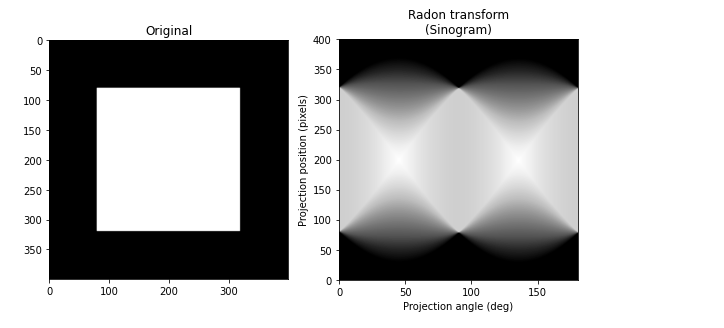
\includegraphics[width=1\textwidth]{figures/a.PNG}

\subsection*{b)}

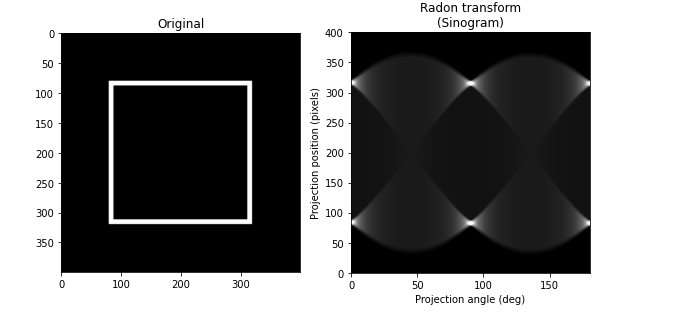
\includegraphics[width=1\textwidth]{figures/b.PNG}